\documentclass{acm_proc_article-sp}
\usepackage[utf8]{inputenc}

\renewcommand{\paragraph}[1]{\vskip 6pt\noindent\textbf{#1 }}
\usepackage{hyperref}
\usepackage{graphicx}
\usepackage{url}

\providecommand{\tightlist}{%
  \setlength{\itemsep}{0pt}\setlength{\parskip}{0pt}}

\title{ShinyPET: A Predictive, Exploratory and Text RShiny Application
using Airbnb data}


% Add imagehandling

\numberofauthors{2}
\author{
\alignauthor Ang Su Yiin \\
        \affaddr{Singapore Management University}\\
       \email{\href{mailto:suyiin.ang.2020@mitb.smu.edu.sg}{\nolinkurl{suyiin.ang.2020@mitb.smu.edu.sg}}}
\and \alignauthor Joey Chua \\
        \affaddr{Singapore Management University}\\
       \email{\href{mailto:joey.chua.2020@mitb.smu.edu.sg}{\nolinkurl{joey.chua.2020@mitb.smu.edu.sg}}}
\and \alignauthor Kevin Gunawan Albindo \\
        \affaddr{Singapore Management University}\\
       \email{\href{mailto:kgalbindo.2019@mitb.smu.edu.sg}{\nolinkurl{kgalbindo.2019@mitb.smu.edu.sg}}}
\and }

\date{}

%Remove copyright shit
\permission{}
\conferenceinfo{} {}
\CopyrightYear{}
\crdata{}

% Pandoc syntax highlighting

% Pandoc citation processing
\newlength{\csllabelwidth}
\setlength{\csllabelwidth}{3em}
\newlength{\cslhangindent}
\setlength{\cslhangindent}{1.5em}
% for Pandoc 2.8 to 2.10.1
\newenvironment{cslreferences}%
  {}%
  {\par}
% For Pandoc 2.11+
\newenvironment{CSLReferences}[3] % #1 hanging-ident, #2 entry spacing
 {% don't indent paragraphs
  \setlength{\parindent}{0pt}
  % turn on hanging indent if param 1 is 1
  \ifodd #1 \everypar{\setlength{\hangindent}{\cslhangindent}}\ignorespaces\fi
  % set entry spacing
  \ifnum #2 > 0
  \setlength{\parskip}{#2\baselineskip}
  \fi
 }%
 {}
\usepackage{calc} % for calculating minipage widths
\newcommand{\CSLBlock}[1]{#1\hfill\break}
\newcommand{\CSLLeftMargin}[1]{\parbox[t]{\csllabelwidth}{#1}}
\newcommand{\CSLRightInline}[1]{\parbox[t]{\linewidth - \csllabelwidth}{#1}}
\newcommand{\CSLIndent}[1]{\hspace{\cslhangindent}#1}

\usepackage{graphicx}
\usepackage{float}
\usepackage{caption}
\captionsetup{skip=1pt}
\setlength{\textfloatsep}{2pt}
\setlength{\intextsep}{2pt}

\begin{document}
\maketitle

\begin{abstract}
The increasing availability of data has resulted in the increased demand
for data driven decisions. Although there is an extensive range of
commercial statistical tools, they are often subscription-based and
demand good technical knowledge to mine and draw insights from.
Therefore, it may not appeal to the average user. Using a collection of
R packages available, ShinyPET, an R-Shiny application is developed for
the average user to perform exploratory and confirmatory analysis, text
mining and predictive analysis, as well as to formulate insights and
make data-driven decisions. Airbnb data provides a baseline for this
application as the data generated is rich in information, consisting of
structured, unstructured, and location data. This paper discusses the
design framework, use case and future works of the ShinyPET dashboard.
\end{abstract}

\emph{Keywords} - Airbnb, Exploratory Analysis, Confirmatory Analysis,
Text Mining, Predictive Analytics, Decision Making, R Shiny, Interactive
Data Visualisation.

\hypertarget{introduction}{%
\section{Introduction}\label{introduction}}

With increasing affordable data storage and processing technologies, the
demand for data-driven decision-making (DDDM)\footnote{DDDM refers to
  the systematic analysis, examination and integration of data to making
  strategic decisions, rather than based on intuition or observation
  alone (Mandinach, 2012)
  {[}\protect\hyperlink{ref-doi:10.1080ux2f00461520.2012.667064}{5}{]}}
has increased significantly. As Geoffrey Moore opines, ``Without big
data analytics, companies are blind and deaf, wandering out onto the Web
like deer on a freeway.'' With the use of data driven decision making
through analytics tools, firms performance would improve (Yasmin, M et
al., 2020)
{[}\protect\hyperlink{ref-https:ux2fux2fdoi.orgux2f10.1016ux2fj.jbusres.2020.03.028}{8}{]}

Airbnb is an online vacation rental maravailableketplace servicing a
community of hosts and travellers. By 2020, Airbnb has millions of
listings in over 220 counties and regions across 100,000 cities
{[}\protect\hyperlink{ref-airbnb2021}{1}{]}. The data generated provides
rich information, including structured data e.g.~price and location, as
well as unstructured data e.g.~reviews and listing descriptions. Thus,
Airbnb provides a good use case and base case for exploratory and
confirmatory analysis, text mining, and predictive modeling as presented
in our ShinyPET dashboard.

\hypertarget{motivation-of-the-application}{%
\section{Motivation of the
application}\label{motivation-of-the-application}}

The motivation of this project stems from two main issues - the
proliferation of data and lack of user-friendly tools to make
data-driven decision. According to Harris (2012)
{[}\protect\hyperlink{ref-harris_2014}{2}{]}, data is impractical
without the ability to analyse it. Although there is a wide range of
commercial statistics and analytics tools, these tools are often
subscription-based and require technical knowledge to mine and draw
insights from. On the other hand, while open source tools as such Python
and R allow for data visualisations, users would require extensive
programming background to generate such insights.

Hence, this project aims to develop an interface which is concise,
interactive, and user-friendly using R Shiny. With this interface,
data-based decisions can be made from the interactive GUI. The R Shiny
App will cover 3 modules: 1) Exploratory - users are able to draw
interesting patterns based on selected variables, which are augmented by
statistical tests based on the chosen variables. 2) Text - users are
able to perform analysis on textual data such as reviews to generate
quantitative insights.\\
3) Predictive - users are able to prepare and build a variety of
prediction models without the need to have in-depth understanding of
predictive models and their algorithms.\\
This application can be extended to Airbnb data from other countries,
and also to other datasets.

\hypertarget{review-and-critic-on-past-works}{%
\section{Review and critic on past
works}\label{review-and-critic-on-past-works}}

Radiant application {[}\protect\hyperlink{ref-radiant2019}{6}{]}, an
open-source platform-independent browser-based interface for business
analytics in R, illustrates the robustness of Rshiny for web-based
application. Developed to promote quick and reproducible data analytics,
the application provides interactivity and flexibility in performing
visualisation, statistical and predictive analysis. However, there are
limitations to the application. First, in terms of exploratory data
analysis, most of the plots produced are of static nature which can be
enhanced by wrapping plotly around them. Secondly, for statistical
testing, users are expected to have a basic understanding of statistical
testing methods as they are first required to select their testing
method, which can be further enhanced by automating testing methods
based on inputs. In addition, newer packages such as visNetwork can be
applied for interactive tree visualisation that in turn improves the
assessment of decision tree model. Lastly, the statistical testing and
charts are placed in separate tabs. In terms of visualisation, a
single-page view would enhance the aesthetics and usability.

Text Mining with R Book {[}\protect\hyperlink{ref-robinson}{7}{]}
authored by Silge and Robinson presents a comprehensive approach to
handle text. First, the book is content-heavy, which may not be
appealing to the typical users. Second, tidytext used for data wrangling
and visualisation is widely used, thus allowing users to apply such
methods easily. However, these tools require technical skills from users
and are not interactive. To allow easy usage and enhance interactivity,
packages such as plotly and highchart can be used. Highcharter has
various themes and features such as tooltips which greatly enhance
visualisation.

Tidymodels {[}\protect\hyperlink{ref-tidymodels2020}{3}{]} has gained
interest by providing a framework for predictive modeling and machine
learning. It is aligned with the tidyverse principles which leads to a
tidier and consistent grammar in the predictive analytics process.
Different models offered in Radiant package are also available for
implementation in Tidymodels framework, which is why our application
leverages Tidymodel as the main framework to conduct predictive
analytics on Airbnb data.

Lu, Y., Garcia, R., Hansen, B. et al.~(2017)
{[}\protect\hyperlink{ref-https:ux2fux2fdoi.orgux2f10.1111ux2fcgf.13210}{4}{]}
provides a comprehensive summary of research on Predictive Visual
Analytics. The paper discusses how visual analytics systems are
implemented to support predictive analytics process such as feature
selection, incremental learning, model comparison and result
exploration. The overall goal of visual analytics is to support
explanation in each step of predictive analytics exercise which is also
our motivation in developing this application.

\hypertarget{design-framework}{%
\section{Design framework}\label{design-framework}}

The design of our shinyPET is based on ensuring a comprehensive data
analysis coupled with aesthetics. Taking into account the user point of
view, 3 main principles, namely user-friendliness, interactivity and
ease of understanding are adopted.

To get started, the introduction page provides an overview of the
application. This allow users to have an understanding of the case that
he/she will be exploring.

In the exploratory module (section 4.1), data summary and their tabular
form would be presented for user's understanding of data. In the explore
sub tab, users are able to visualise provided data based on various
variables. This user-friendliness and interactivity provides flexibility
and ease of use without needing any technical knowledge. In the text
module (section 4.2), various text mining technique tools are presented.
Each sub tab utilises visusaliation tools like word clouds and topic
modeling to simplify concepts in natural language processing. This aids
in understanding of the unstructured data provided. In the predictive
module (section 4.3), various predictive models are available for user
selection. The sub tabs guide users through the process from data
sampling to final model selection. Visualisation and interactivity are
embedded through graphs and user input menu to provide an organised
workflow of predictive analytics. Aesthetically, the application's
colour scheme should be based on the theme of the topic. Using our case
of Airbnb, the official colours are Raush, Babu and Foggy (type of
gray).

The combination of the 3 principles are consistently incorporated into
various steps of the data analysis in the 3 modules, hence providing
users an easy and comprehensive way to make data-driven decisions.

\hypertarget{exploratory-module}{%
\subsection{Exploratory module}\label{exploratory-module}}

The exploratory module enables users to perform Exploratory Data
Analysis (EDA) and Confirmatory Data Analysis (CDA) on selected
variables to identify interesting patterns. There are three sections in
this module - observe, map and confirm \& explore.

\hypertarget{observe-submodule}{%
\subsubsection{Observe submodule}\label{observe-submodule}}

In Figure 1, the Observe section provides a summary of the data to
facilitate users to understand and form questions surrounding the data.

\begin{figure}[H]

{\centering 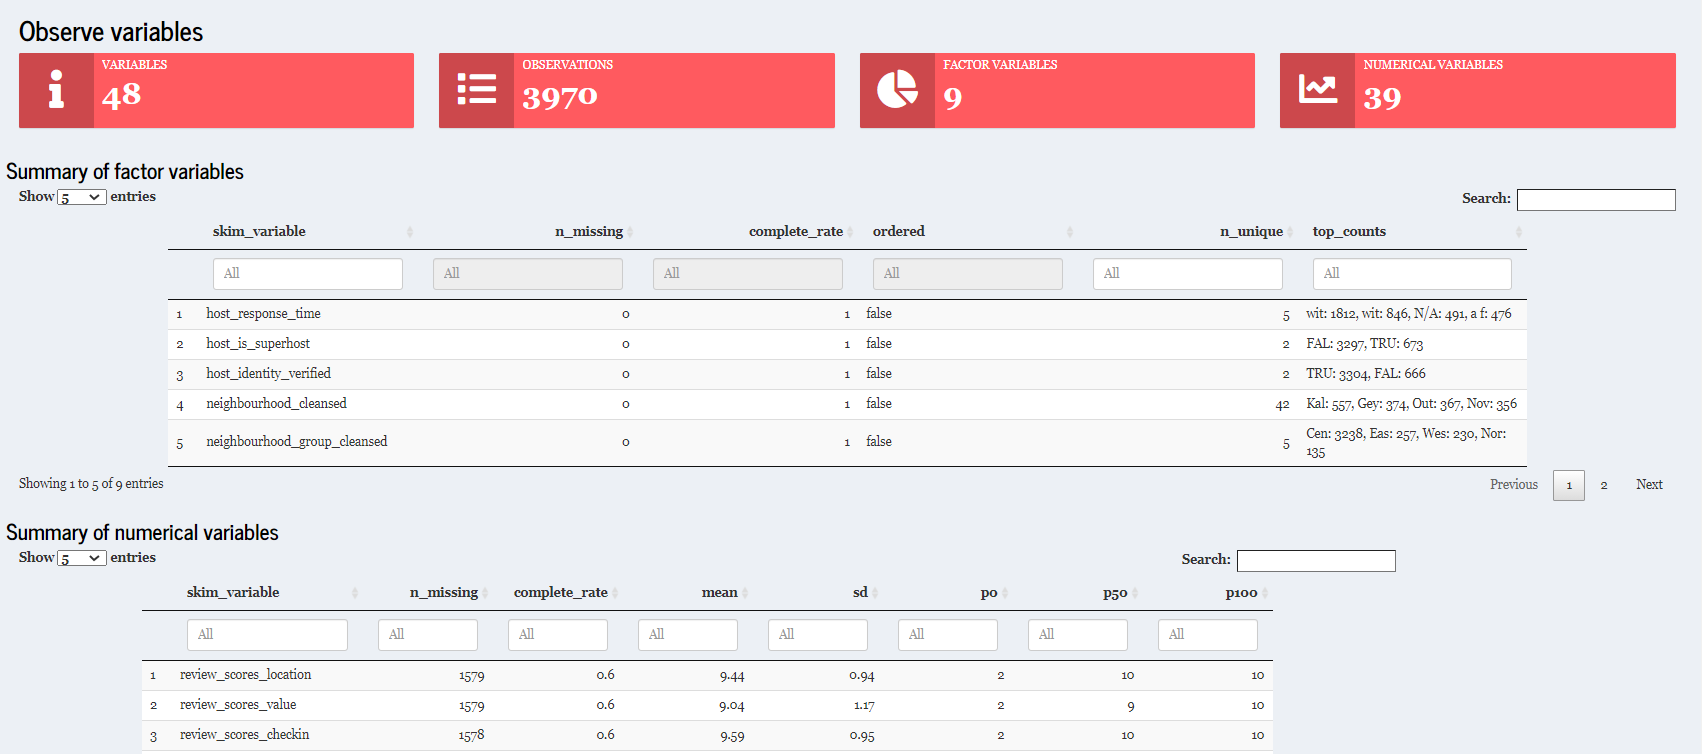
\includegraphics[width=1\linewidth]{images/design_observe} 

}

\caption{Interface and components of Observe section}\label{fig:unnamed-chunk-1}
\end{figure}

2 main components are presented in this section. The first component is
the 4 boxes at the top of the page, which present an overview of the
data by showing the number of variables, observations and data types.
The second component is the summary of each variable according to their
data types in a tabular format. Users are able to use the search boxes
to filter data, and use the arrow icons to sort data. Hence, these
components incorporate both ease of understanding and interactivity.

\hypertarget{map-submodule}{%
\subsubsection{Map submodule}\label{map-submodule}}

Figure 2 shows the Map section that allows user to explore the
geographic patterns through thematic maps. The maps are designed based
on the three principles stated above and partially on Shneiderman's
interactive dynamics principle of ``overview, zoom and filter, then
details on demand.'' `zoom and filter' portion were not used as they are
not applicable to this dataset.

\begin{figure}[H]

{\centering 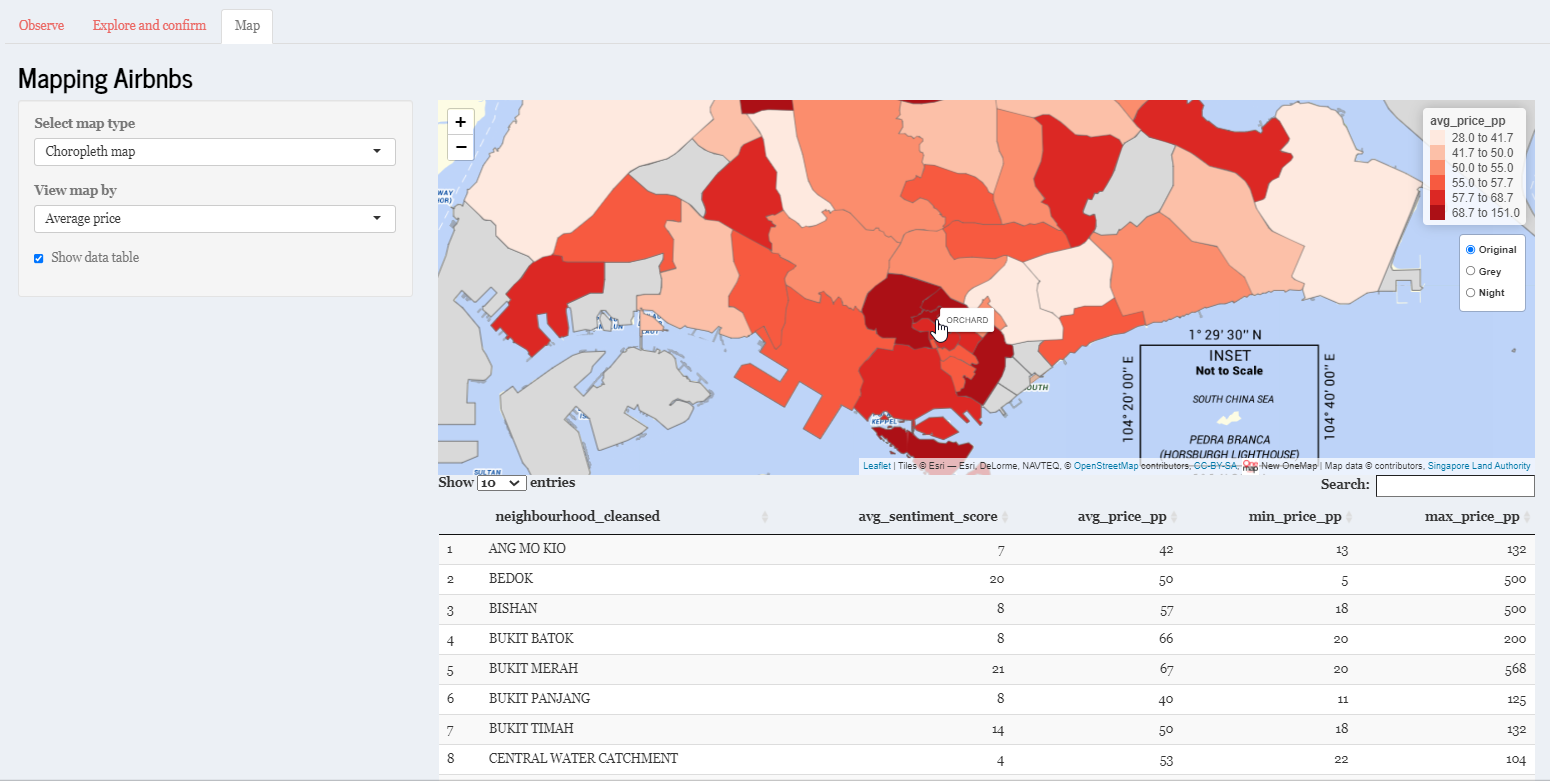
\includegraphics[width=1\linewidth]{images/design_map} 

}

\caption{Interface and components of Map section}\label{fig:unnamed-chunk-2}
\end{figure}

There are 2 main components to submodule - the map which consist of
bubble map and cloropleth map, and the table, which provides details of
the map. These maps are chosen as they are deemed to fit the
understanding of the data. For instance, price and review scores are
used to show the price and score ranges spread shown by the intensity of
the colour.

\hypertarget{explore-and-confirm-submodule}{%
\subsubsection{Explore and confirm
submodule}\label{explore-and-confirm-submodule}}

Figure 3 shows the EDA and CDA submodule for users to explore and
perform inferential statistics based on the section 4.1.1 and 4.1.2.

\begin{figure}[H]

{\centering 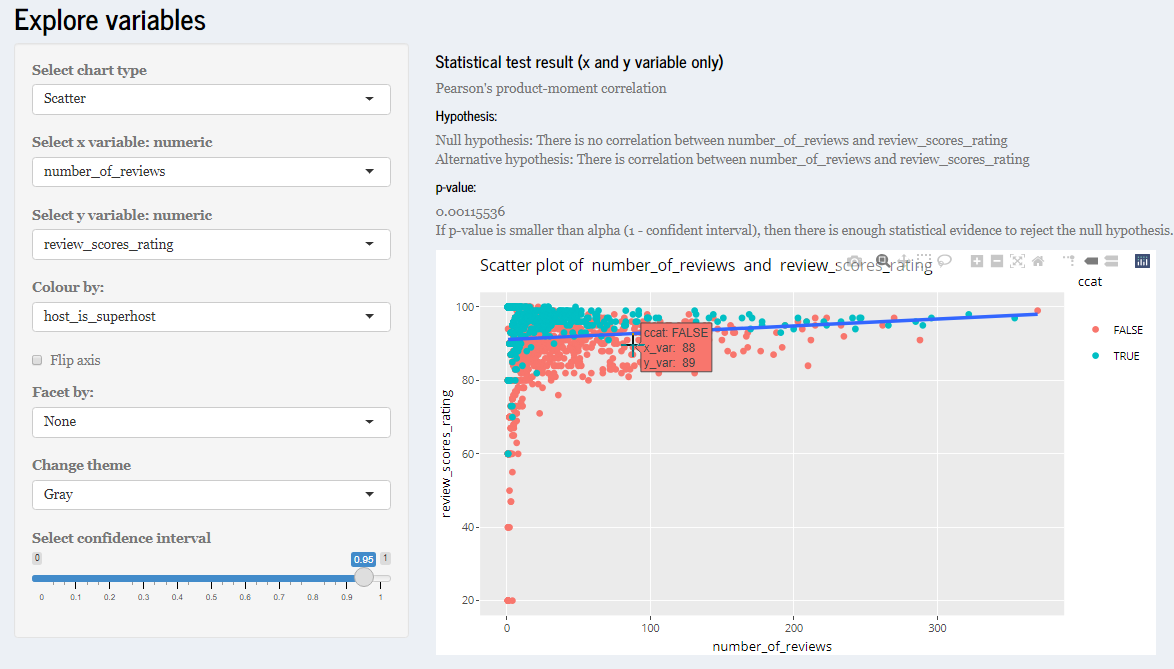
\includegraphics[width=1\linewidth]{images/design_explore1} 

}

\caption{Interface and components of Explore and Confirm section}\label{fig:unnamed-chunk-3}
\end{figure}

There are 3 main components - the selection input on the left, the
statistical results and the chart. The selection input with drop-down
list allow users to customise charts shown. The application provides for
4 types of chart namely: distribution, mosaic, boxplot and scatter plot.
Based on the selection input, drop-down menus for variables will be
altered accordingly. For example, if `Distribution' chart was selected,
only the x-variable drop-down input will be shown.

The chart was designed based on Shneiderman's interactive dynamics of
highlight, filter or manipulate. This graphs allows users to manipulate
views by selecting an object in a plot, highlighting selected records
and defining a region on the graph. Furthermore, the plotted charts can
be downloaded for users to communicate their findings. An example of
output is shown in figure 4.

\begin{figure}[H]

{\centering 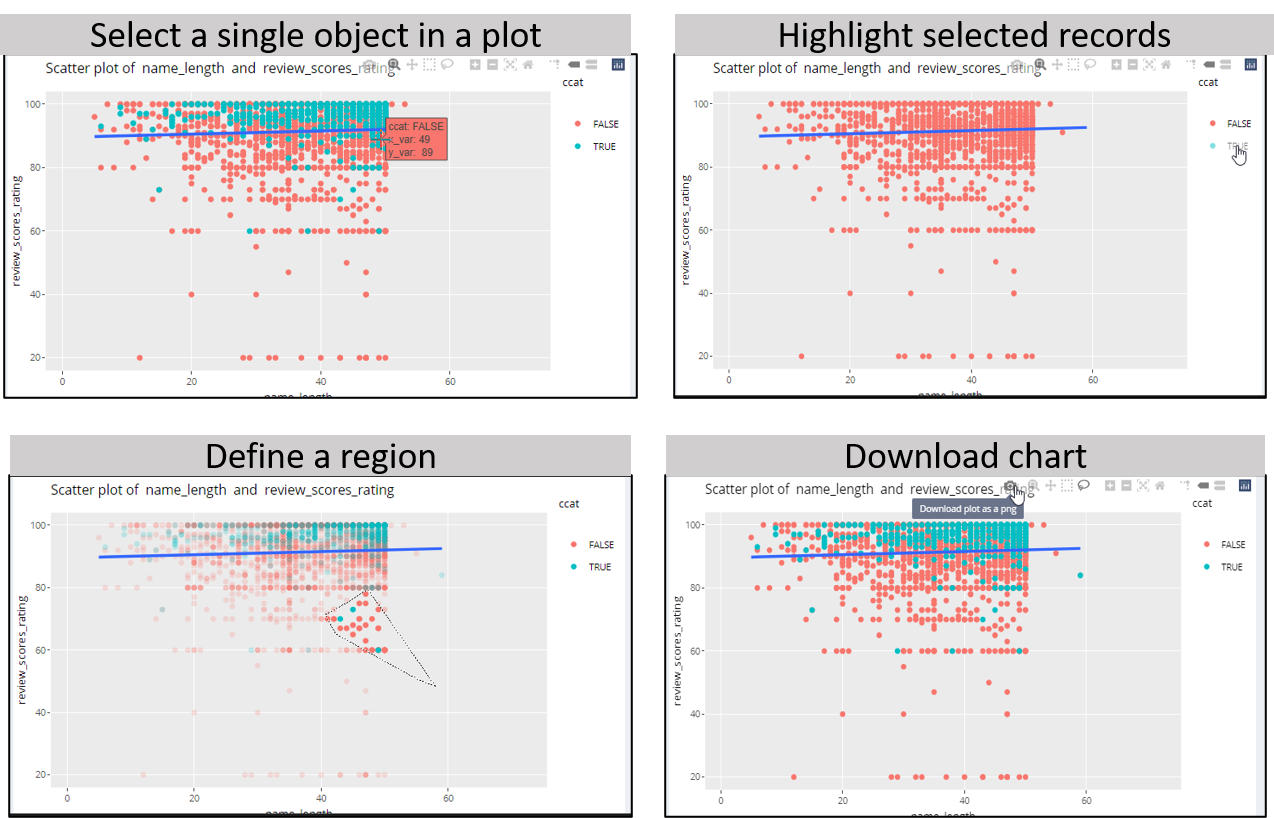
\includegraphics[width=1\linewidth]{images/design_explore2} 

}

\caption{Graph's manipulation function of the Explore and Confirm section}\label{fig:unnamed-chunk-4}
\end{figure}

As the application is tailored towards users that are not well-versed in
statistics, the statistical tests where test methods and results are
automated based on the selected variables, are easy to understand. An
interactive slider is also provided for user to easily adjust
statistical results.

\hypertarget{text-module}{%
\subsection{Text module}\label{text-module}}

The text module utilises various text mining techniques to transform
unstructured text i.e.~reviews into structured format to identify
patterns and bring about meaningful insights.

Prior to application of text mining techniques, text preprocessing has
to be carried out. This involves the use of tokenisation, stemming and
lematisation. Tokenisation is the process of splitting a column of
reviews into tokens such that they are flattened into the format of
one-token-per-row. Stemming is the process of separating the prefixes
and suffixes from words to derive the root word form and meaning.
Stemming algorithms work by cutting off the end or the beginning of the
word, taking into account a list of common prefixes and suffixes that
can be found in an inflected word. Lemmatization, on the other hand,
takes into consideration the morphological analysis of the words.

\hypertarget{token-frequency-submodule}{%
\subsubsection{Token frequency
submodule}\label{token-frequency-submodule}}

To visualise token frequency, wordcloud is used. Worldcloud provides an
easy way to show how frequent a word appears in a corpus. In wordcloud,
the size of a word indicates how frequent the word appears in a given
text.

Other than considering words as individual units, ``ngrams'' are also
used to tokenise pairs of adajacent words. ngrams provide context in
sentiment analysis. For instance, while the word ``happy'' can be
positive, in a sentence which containts the words ``not happy'' would
mean otherwise. Hence, performing sentiment analysis on bigram allow us
to examine sentiment-associated words.

\begin{figure}[H]

{\centering 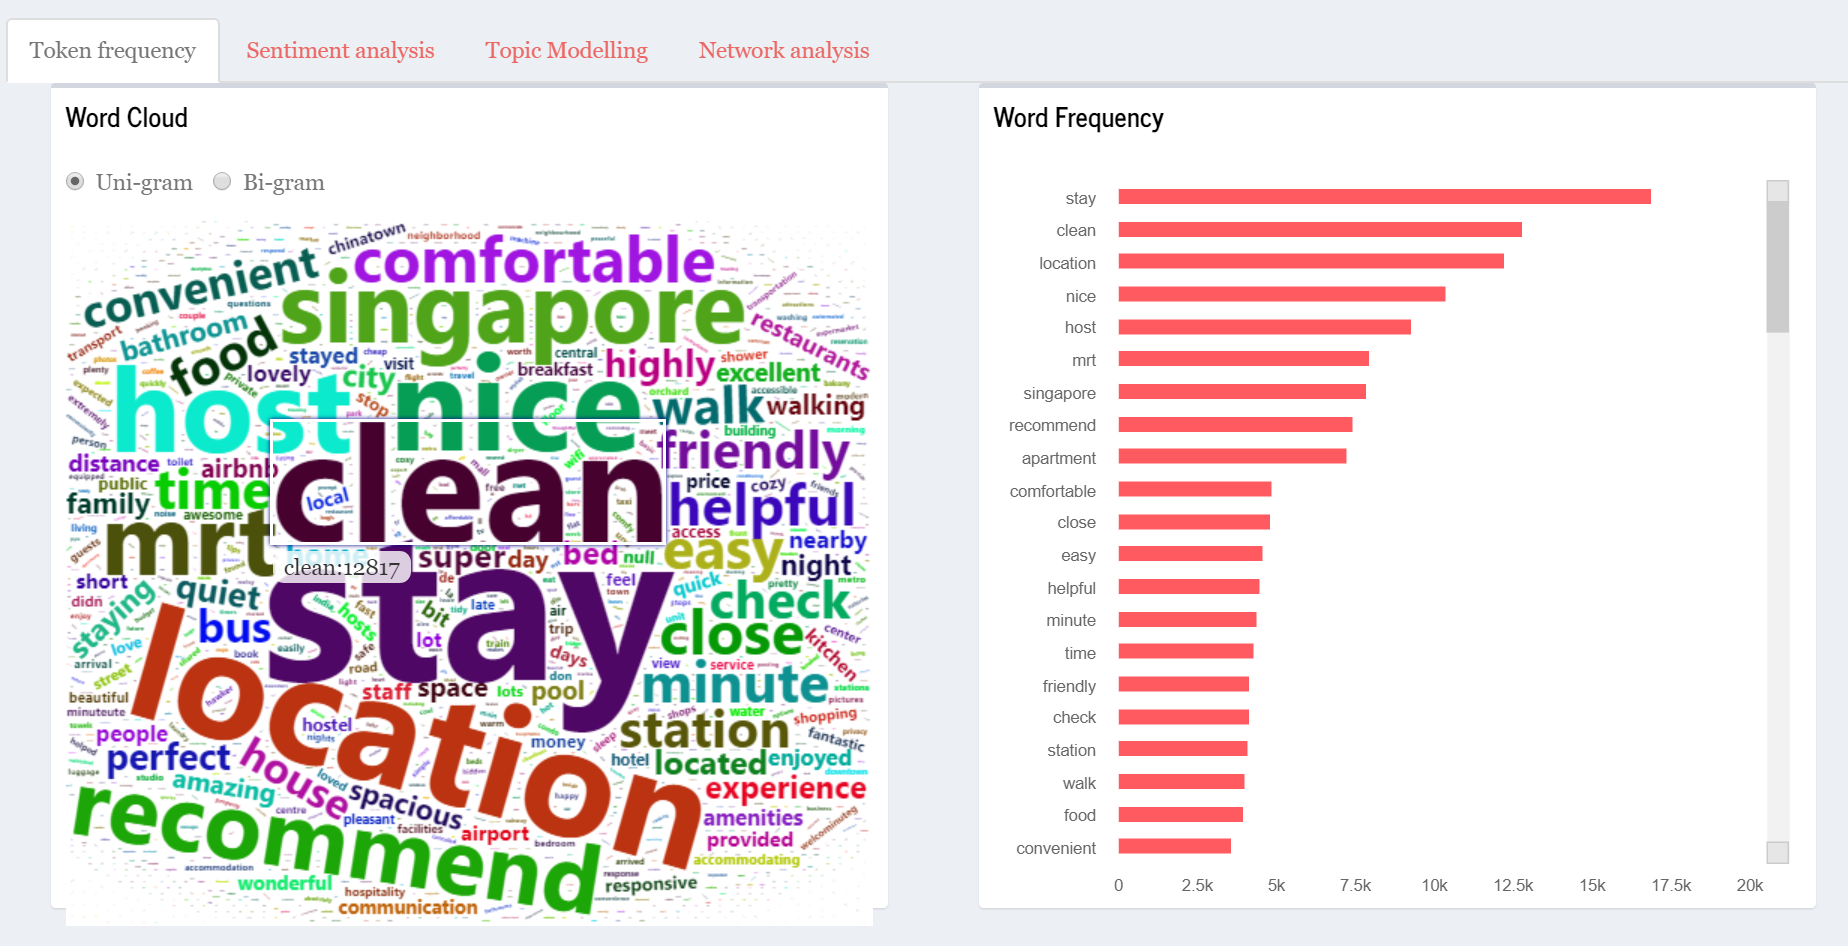
\includegraphics[width=1\linewidth]{images/tokenfrequency} 

}

\caption{Token Frequency}\label{fig:unnamed-chunk-5}
\end{figure}

There are two components: on the left is the wordcloud, and on the right
is the bar chart the ranks the frequency of word in descending order.
From the chart, it can be observed that the words ``clean,'' ``stay,''
``location,'' and ``nice'' occurred most frequently. When ``bi-gram'' is
chosen, the wordcloud and bar chart changes accordingly. Tooltip to show
the number of times the word occurred when hover over allows users to
have understanding of the data. Hence, ease of understanding and
interactivity are prominent.

\hypertarget{sentiment-analysis-submodule}{%
\subsubsection{Sentiment analysis
submodule}\label{sentiment-analysis-submodule}}

In this sub module, 3 dictionaries were used to plot wordcloud that
shows both the frequency and sentiments. AFINN lexicon measures
sentiment with a numeric score between -5 to 5, BING categorises words
as either positive or negative, and NRC categorises words into 8 basic
emotions (anger, fear, anticipation, trust, surprise, sadness, joy, and
disgust) and 2 sentiments (negative and positive).

\begin{figure}[H]

{\centering 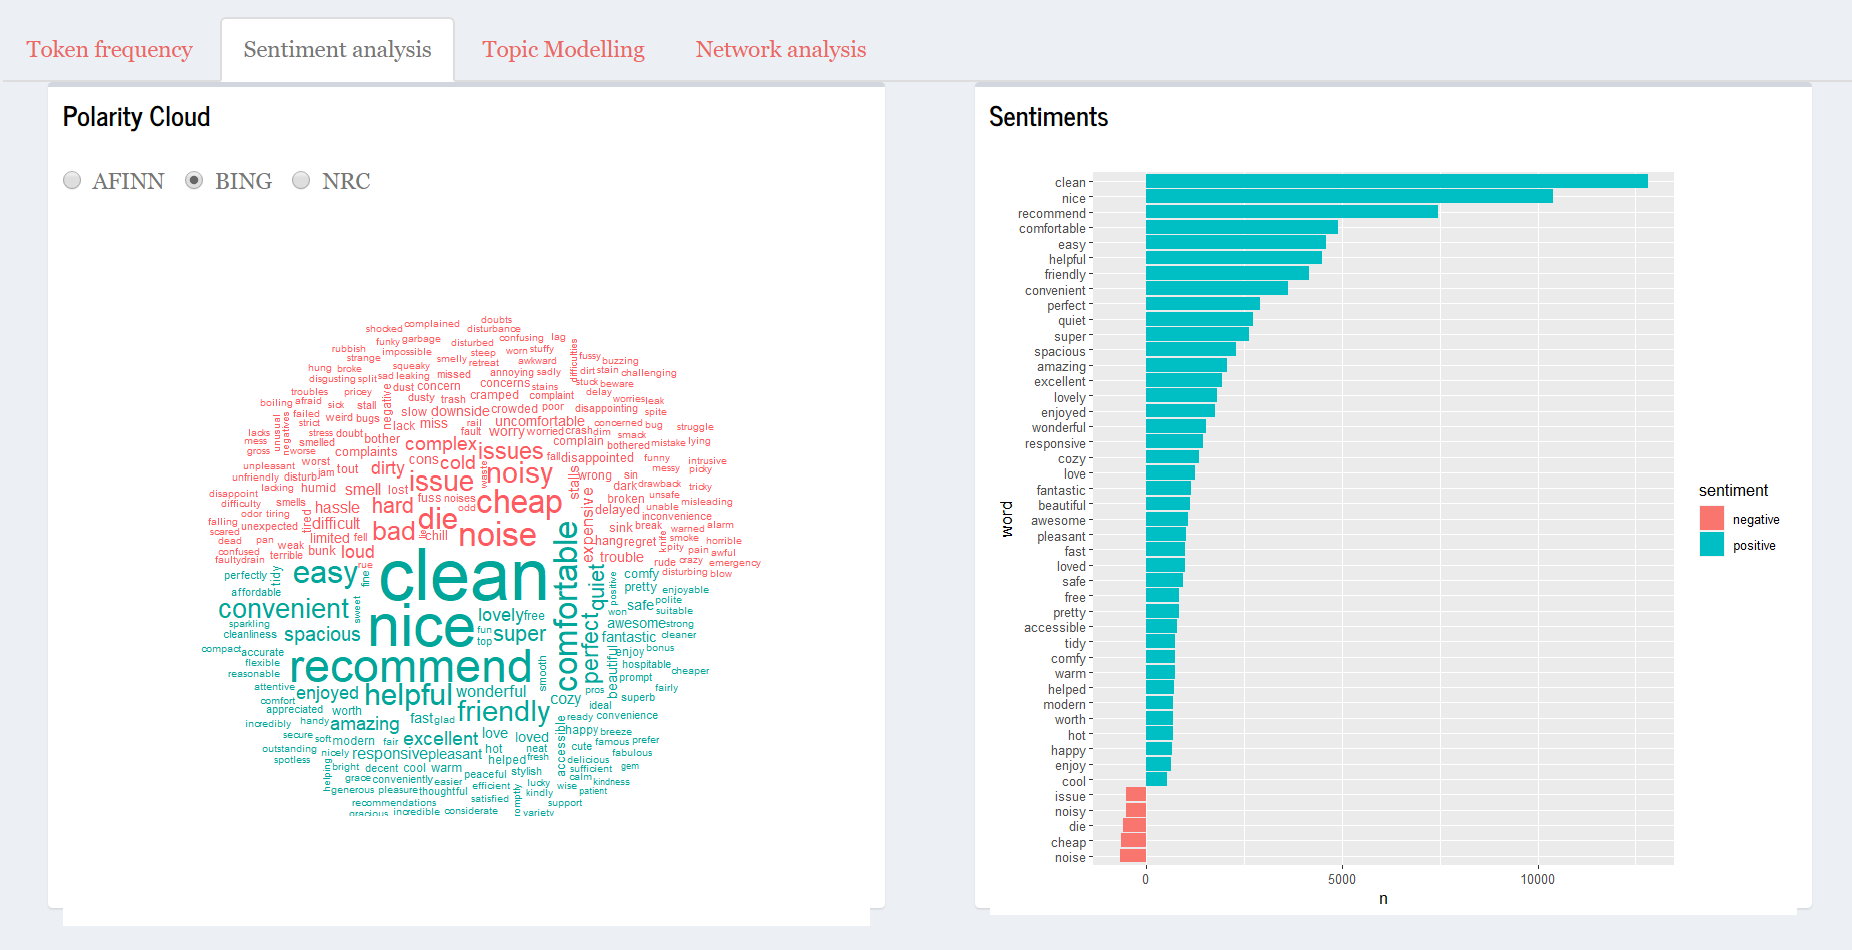
\includegraphics[width=1\linewidth]{images/bingsentiment} 

}

\caption{Sentiment Analysis}\label{fig:unnamed-chunk-6}
\end{figure}

Users can select the various lexicons to view the wordcloud and related
charts such as bar charts and radial chart. For AFINN and BING, bar
charts are plotted to show the spread and weightage of sentiments. For
NRC, a radial plot to show the tendency for reviews to lean towards.

\hypertarget{topic-modelling-submodule}{%
\subsubsection{Topic modelling
submodule}\label{topic-modelling-submodule}}

Latent Dirichlet allocation (LDA) is an example of topic modeling
algorithm, based on 2 principles: First, every document is a mixture of
topics. Second, every topic is a mixture of words.

\begin{figure}[H]

{\centering 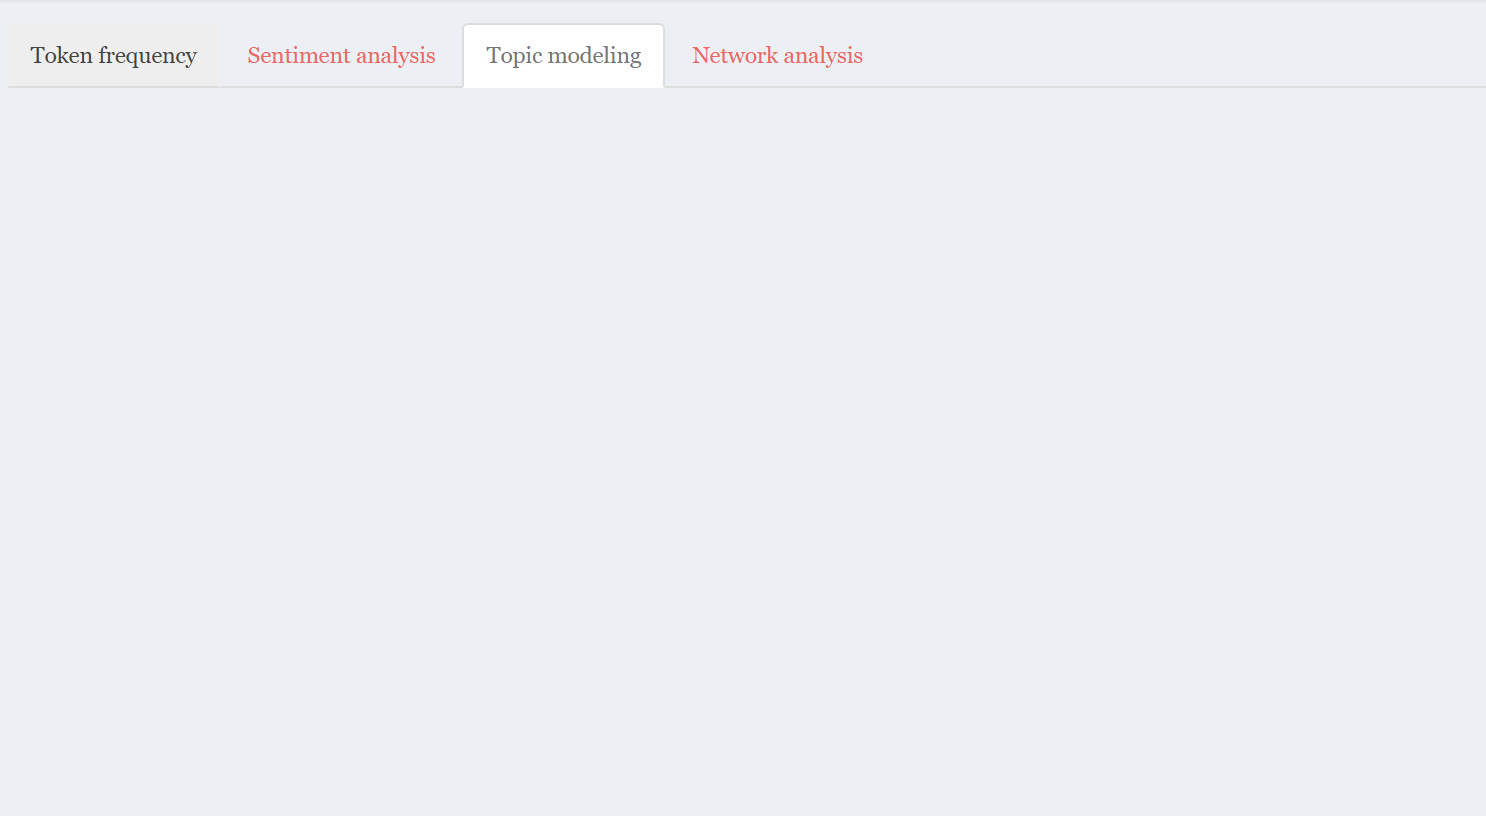
\includegraphics[width=1\linewidth]{images/topicmodelling} 

}

\caption{Topic Modelling}\label{fig:unnamed-chunk-7}
\end{figure}

For flexibility, slider is incorporated to allow users to choose the
number of topics and top terms of the topic. As the loading time is
long, a ``Go'' button is included for users to proceed. Subsequently, 2
components are shown. First, the intertopic distance map that uses
multidimensional scaling algorithm to plot the topics that have words in
common. Second, the bar chart on the right shows salient terms. THe bars
exhibit the total frequency of the term.

\hypertarget{correlation-network-submodule}{%
\subsubsection{Correlation network
submodule}\label{correlation-network-submodule}}

Word occurrences and correlations are commonly used to identify family
of words.

\begin{figure}[H]

{\centering 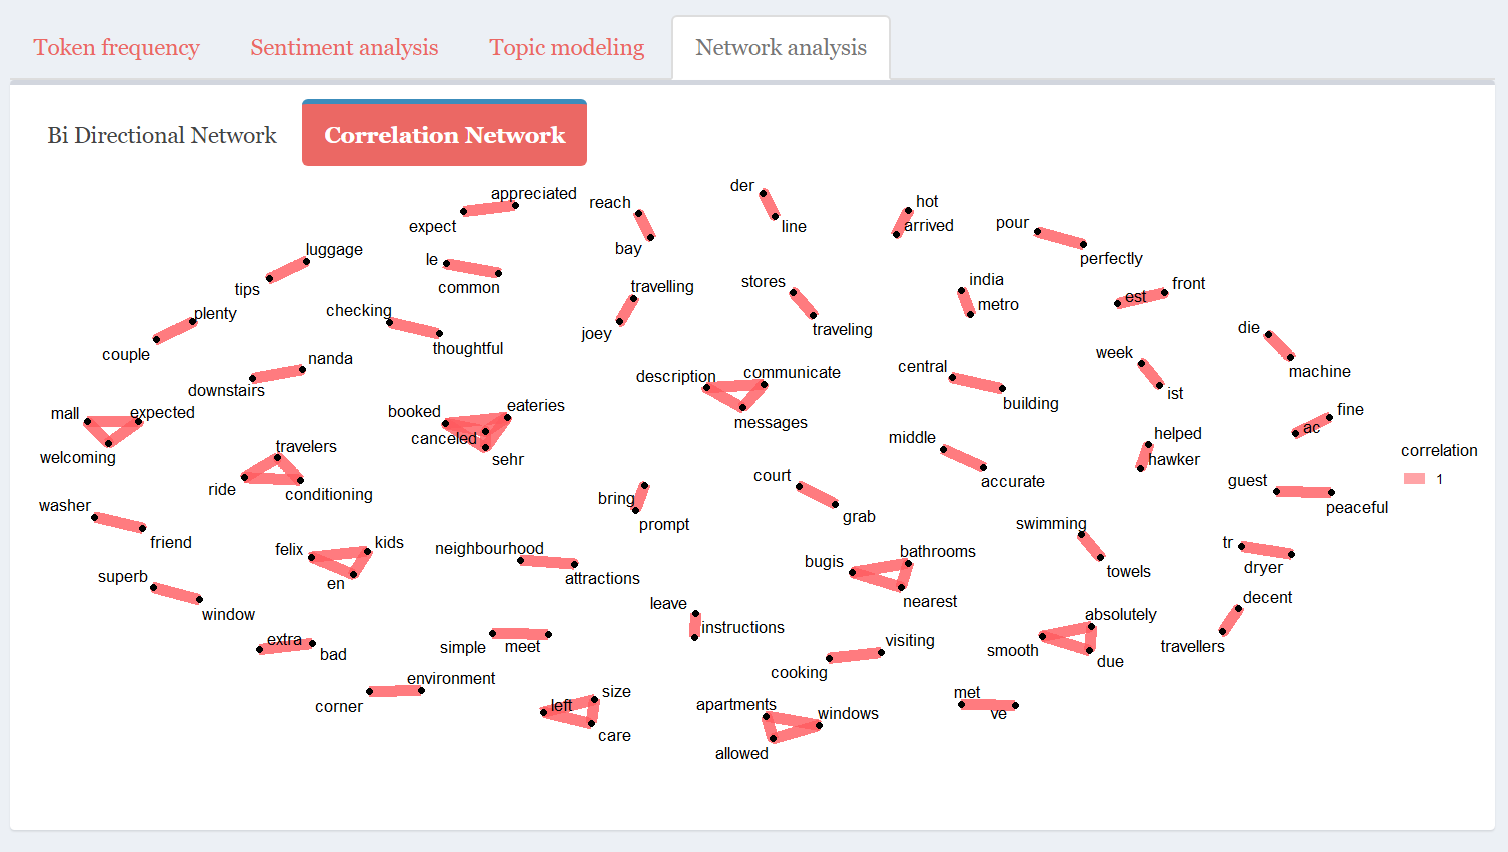
\includegraphics[width=1\linewidth]{images/correlationnetwork} 

}

\caption{Network Analysis}\label{fig:unnamed-chunk-8}
\end{figure}

There are 2 options. First the is Bi-directional Network graph. Second
is the Correlation Network graph. These graphs show how words relate to
each other.

\hypertarget{predictive-module}{%
\subsection{Predictive module}\label{predictive-module}}

The predictive module design framework follows the Tidymodels framework
for data pre-processing, model training, tuning, and validation. On top
of that, feature selections are supported by other R packages such as
ggcorplot (for correlation matrix), ranger and Boruta (for feature
importance). The visualisations and interactivities are embedded in each
step of predictive analytics as explained below.

\hypertarget{data-sampling-submodule}{%
\subsubsection{Data sampling submodule}\label{data-sampling-submodule}}

In this submodule, selection of training-test split proportion provides
user with flexibility in deciding how to spend data budget on the model
development process. The distribution plot between training and test set
displayed highlights potential biases in the training data set.

\begin{figure}[H]

{\centering 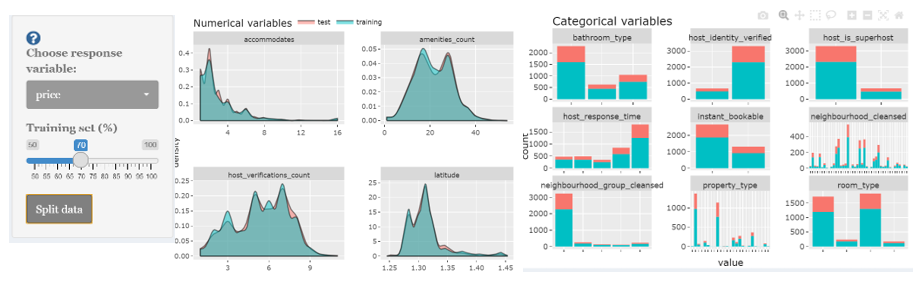
\includegraphics[width=1\linewidth]{images/datasplit} 

}

\caption{Data sampling and distribution plot}\label{fig:unnamed-chunk-9}
\end{figure}

\hypertarget{feature-selection-submodule}{%
\subsubsection{Feature selection
submodule}\label{feature-selection-submodule}}

To support user with selection of variables, correlation matrix with
customised correlation type and p-value criteria are provided. In
addition, variable importance score from 2 different methods highlight
useful predictors towards response variable.

\begin{figure}[H]

{\centering 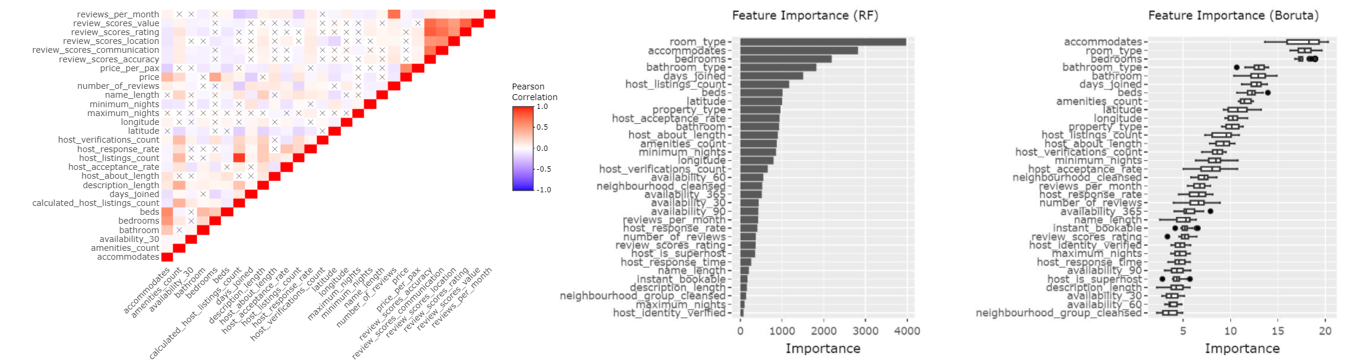
\includegraphics[width=1\linewidth]{images/featselect} 

}

\caption{Correlation matrix and variable importance}\label{fig:unnamed-chunk-10}
\end{figure}

\hypertarget{data-transformation-submodule}{%
\subsubsection{Data transformation
submodule}\label{data-transformation-submodule}}

Prior to training, transformation steps are performed using recipe
package in Tidymodel. Following transformation steps, plot between pre
and post processing step is added to increase user awareness on what
transformation steps are performed and on which variables.

\begin{figure}[H]

{\centering 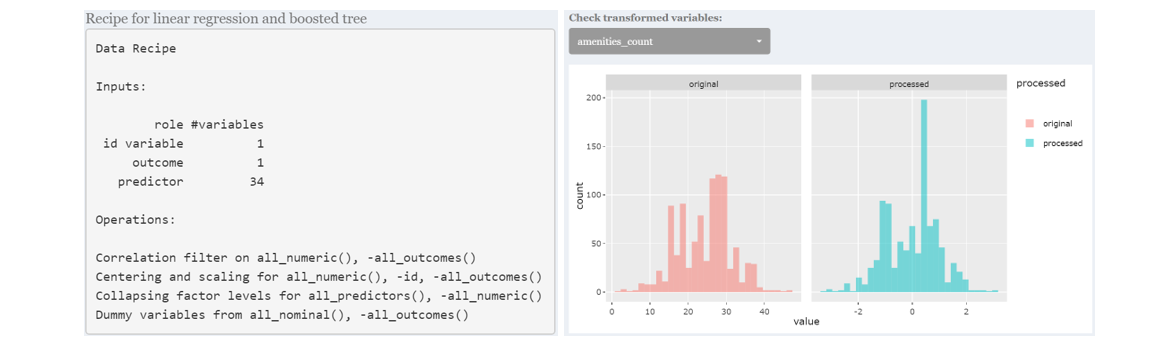
\includegraphics[width=1\linewidth]{images/recipetrf} 

}

\caption{Data transformation steps}\label{fig:unnamed-chunk-11}
\end{figure}

\hypertarget{model-training-submodule}{%
\subsubsection{Model training
submodule}\label{model-training-submodule}}

In this sub module, user can select from 5 different types of predictive
models for training. For linear regression model, coefficient estimates
are shown with option to filter important variables based on p-value.
For decision tree training result, visNetwork package is used for its
decision tree plot to improve result evaluation.

\begin{figure}[H]

{\centering 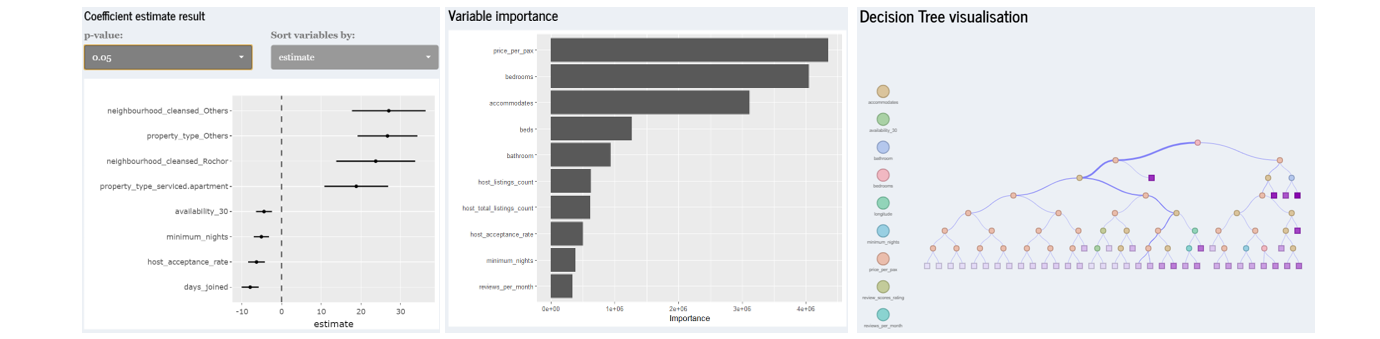
\includegraphics[width=1\linewidth]{images/mdltrn} 

}

\caption{Training result evaluation}\label{fig:unnamed-chunk-12}
\end{figure}

Following, trained model is assessed using test set (unseen data) which
is in turn assessed by plotting the actual and predicted value on an
Rsquare plot. Table of metric performances such as root mean square,
mean absolute error, and Rsquare value is also displayed

\begin{figure}[H]

{\centering 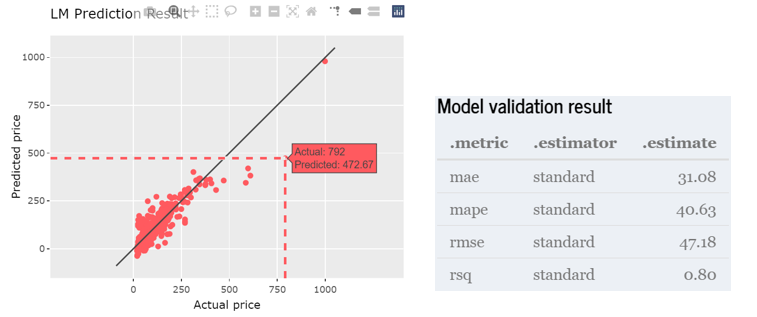
\includegraphics[width=1\linewidth]{images/mdleval} 

}

\caption{Validation result evaluation}\label{fig:unnamed-chunk-13}
\end{figure}

For linear regression model, users have an option to further evaluate
cases with high prediction error. Training set distribution plot is
overlapped with predicted values, which may highlight outliers in the
predictors. Users can also choose to show N number of top predictor
based on p-value score to be displayed.

\begin{figure}[H]

{\centering 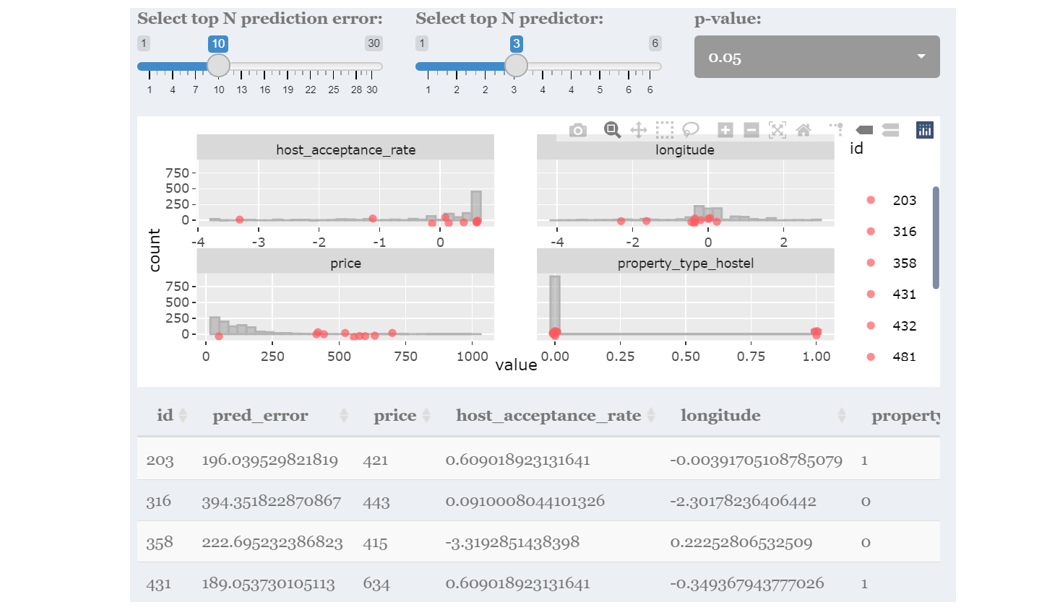
\includegraphics[width=1\linewidth]{images/prederror} 

}

\caption{Prediction error assessment}\label{fig:unnamed-chunk-14}
\end{figure}

Tree based model and generalised linear model use cross validation
training set to tune the model's hyper-parameter. Plot of model
performance using different hyper-parameters settings are available for
user to understand the change in performance.

\begin{figure}[H]

{\centering 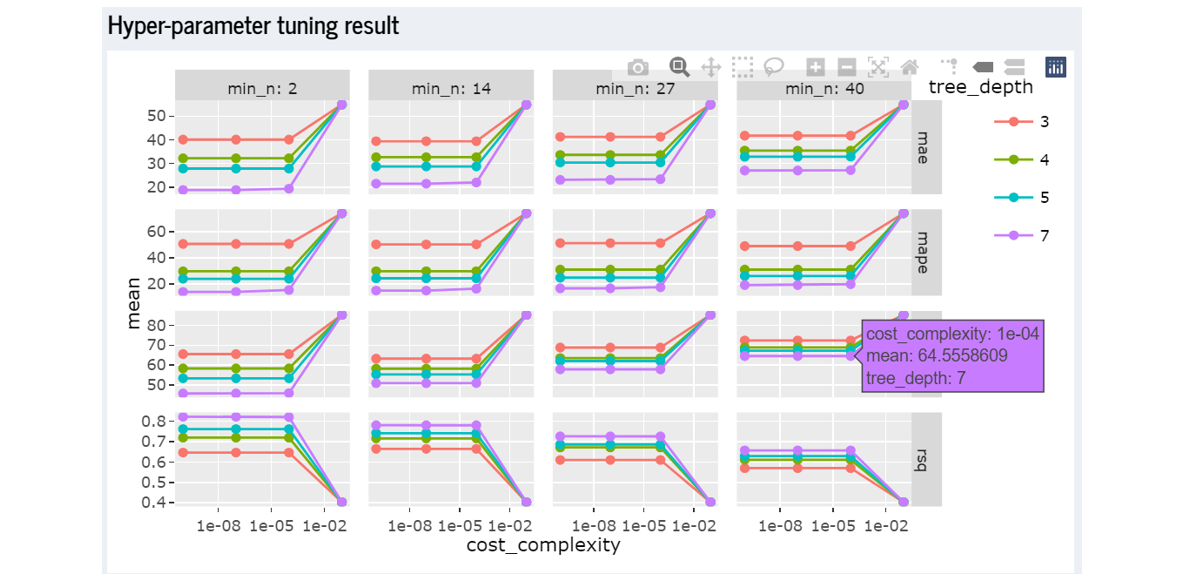
\includegraphics[width=1\linewidth]{images/hypartune} 

}

\caption{Hyper-parameter tuning result}\label{fig:unnamed-chunk-15}
\end{figure}

\hypertarget{model-selection-submodule}{%
\subsubsection{Model selection
submodule}\label{model-selection-submodule}}

In the final submodule, all trained and validated models are gathered
and their metrics are compared for user to choose the final model. Once
selected, user will be able to provide new input variables to each
predictor and get the response variable using the selected model.

\begin{figure}[H]

{\centering 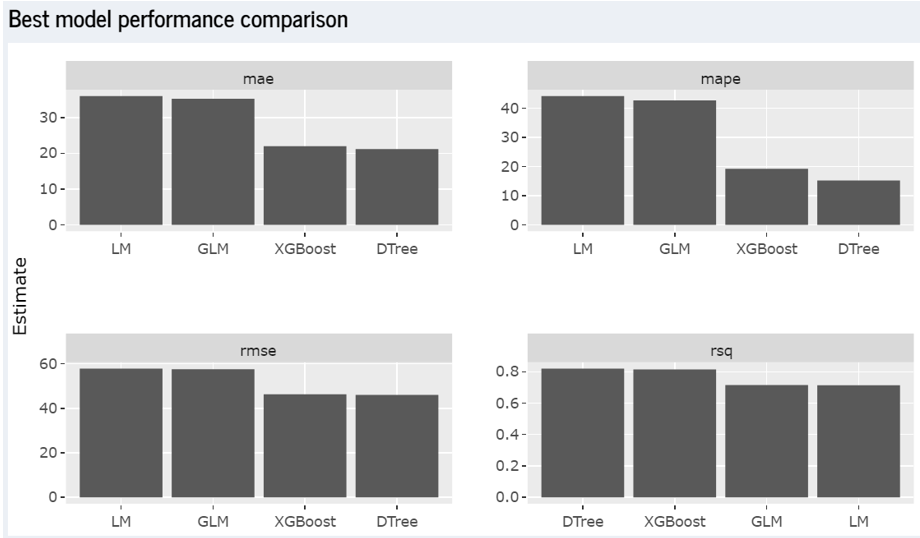
\includegraphics[width=1\linewidth]{images/mdlcompare} 

}

\caption{Models performance comparison}\label{fig:unnamed-chunk-16}
\end{figure}

The combination of these three modules, along with its interactivity and
usability would empower users to make data-driven decisions based on the
insights generated.

\hypertarget{case-study-airbnb-singapore}{%
\section{Case Study : Airbnb
Singapore}\label{case-study-airbnb-singapore}}

InsideAirbnb provides tools and data for users to explore Airbnb. 2
files dated 27 January 2021 were used: (1) listing.csv.gz: This dataset
consists of 74 variables and 4256 data points (2) reviews.csv.gz: This
dataset provides 6 variables and 52368 data points. Our application can
be used from both the perspective of hosts and guests.

\textbf{Hosts}: In 2014, Airbnb launched the Superhost programme to
reward hosts with outstanding hospitality. As a Superhost, one will have
better earnings, more visibility, and are able to earn exclusive rewards
such as increased earnings compared to regular hosts. To become a
Superhost, these are the criteria to be met: - 4.8 or higher overall
rating based on reviews - Completed at least 10 stays in the past year
or 100 nights over at least 3 completed stays - Less than 1\%
cancellation rate, not including extenuating circumstances - Responds to
90\% of new messages within 24 hours \textbf{Guests}: With over 60,000
members and 6,000 properties listed on Airbnb website, a dilemma on
which is the right space might be of concern to users. Various modules
in our dashboard will allow both types of users to analyse Airbnb data
according to their needs.

In order to reduce the loading time of the application, the datasets
were preprocess and only the cleaned datasets were loaded. In addition,
redundant variables such as listing id, url id, were removed.

\hypertarget{geographical-distribution-of-airbnbs}{%
\subsection{Geographical distribution of
Airbnbs}\label{geographical-distribution-of-airbnbs}}

The point symbol map reveals that the distribution of Airbnb listings in
Singapore has high concentration in the central regions. The 4 distinct
hotspots are (1) Geylang/Kallang, (2) Lavender/ Rochor / Bugis, (3)
Orchard and (4) Chinatown. Area (3) and (4) are mainly tourist areas -
(3) Orchard is the main shopping belt of Singapore and (4) Chinatown
retains significant historical and cultural landmarks. Areas (1) and (2)
are popular given their low prices per person (see choropleth map on the
right) while staying relatively close to central. Additionally, Airbnb
listings tend to be located along the MRT station track, which could
signify the use of public transports are generally more popular for
Airbnb guests.

\begin{figure}[H]

{\centering 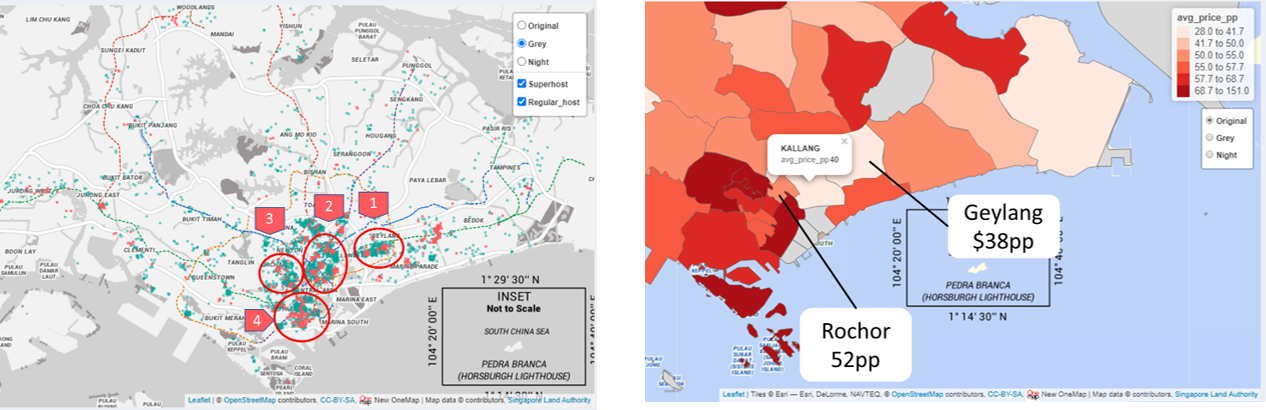
\includegraphics[width=1\linewidth]{images/usecase_explore} 

}

\caption{Point symbol map on the left, choropleth on the right}\label{fig:unnamed-chunk-17}
\end{figure}

With this information, potential Airbnb investors can identify highly
saturated areas and the average price per person of that area, which
could help in estimatation of their investment yield prior to commitment
of investments.

\hypertarget{distribution-of-review-score-rating}{%
\subsection{Distribution of review score
rating}\label{distribution-of-review-score-rating}}

The overall Airbnb listing review score - `review\_scores\_rating,' is
capped at 100 and has a left-skewed distribution. This suggests that
most guests tend to post positive reviews, or listings with low ratings
tend to be delisted/exited from Airbnb market.

\begin{figure}[H]

{\centering 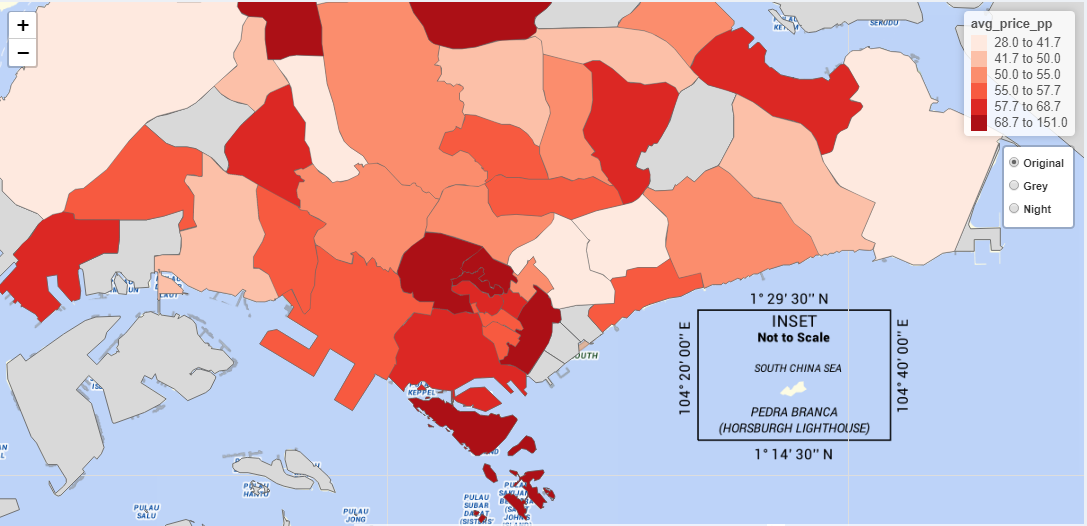
\includegraphics[width=1\linewidth]{images/usecase_explore2} 

}

\caption{Distribution of review score rating}\label{fig:unnamed-chunk-18}
\end{figure}

\hypertarget{confirmatory-analysis-of-superhost-and-review-scores-hosting}{%
\subsection{Confirmatory analysis of superhost and review scores
hosting}\label{confirmatory-analysis-of-superhost-and-review-scores-hosting}}

The chart below suggests that listings with the superhost status tend to
have higher review scores as indicated the statistical test results
where p-value is less than alpha of 0.05.

\begin{figure}[H]

{\centering 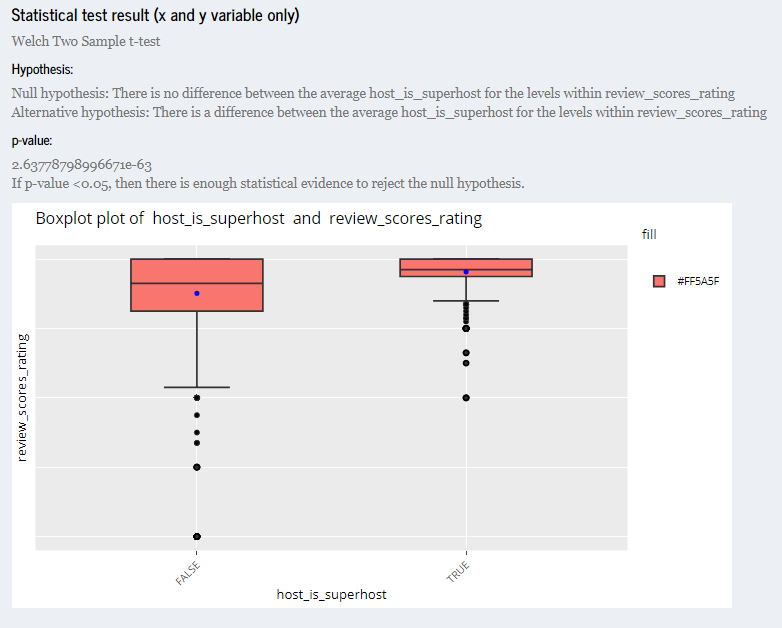
\includegraphics[width=1\linewidth]{images/usecase_explore4} 

}

\caption{Exploratory and Confirmatory Analysis on superhost status and review scores}\label{fig:unnamed-chunk-19}
\end{figure}

\hypertarget{observing-correlation-among-variables}{%
\subsection{Observing correlation among
variables}\label{observing-correlation-among-variables}}

Data sets like Airbnb are rich with large numbers of variable. However,
multicolinearity among variables are known to affect predictive model
performance. Correlation matrix helps to identify multicolinearity by
highlighting variables with high correlation value. In our example
below, we observe correlations within rating score components, listing
availability period, and review components. With this information,
selection of variables can be done properly.

\begin{figure}[H]

{\centering 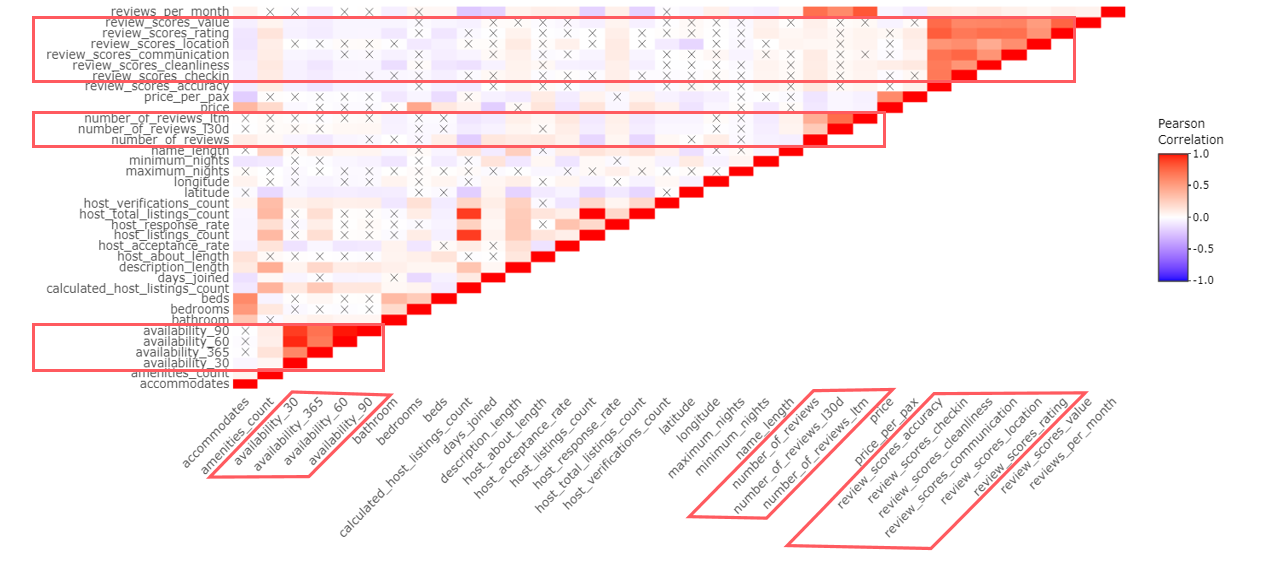
\includegraphics[width=1\linewidth]{images/corrcase} 

}

\caption{Correlation among variables}\label{fig:unnamed-chunk-20}
\end{figure}

\#\#Sentiment Analysis From the wordclouds and polarity clouds, the
cleanliness of room seem to be mentioned the most frequently.
Additionally, the distance to various areas and transport based on words
like ``minute walk,'' ``bus stop,'' and ``public transport'' seemed to
play an important factor to providing ratings and review. Based on the
various lexicons, there is a common result of sentiments being skewed
towards the positive side.

\hypertarget{model-explanation}{%
\subsection{Model Explanation}\label{model-explanation}}

In predicting listing price using linear model, the plot of coefficient
estimate helps to explain the trained model. In the example below, our
interface allows sorting of variables based on p-value score where
variables with lowest p-value is located on top. Property type which
falls under ``Others'' category (those with counts of less than 5\% in
the data set) has the lowest p-value score and positive estimate, which
may represent unique property type (e.g.~boat, campsite, chalet, villa)
where the listing price is above the average price of common property
type like apartment and condominium (as shown in the boxplot from
exploratory module). Amenities and beds are also in the top 5 predictor
where it correlates positively with listing price. However, the error
bar is wider for property type ``Others'' as compared to the amenities
and beds, representing more uncertainty in the estimate value.

\begin{figure}[H]

{\centering 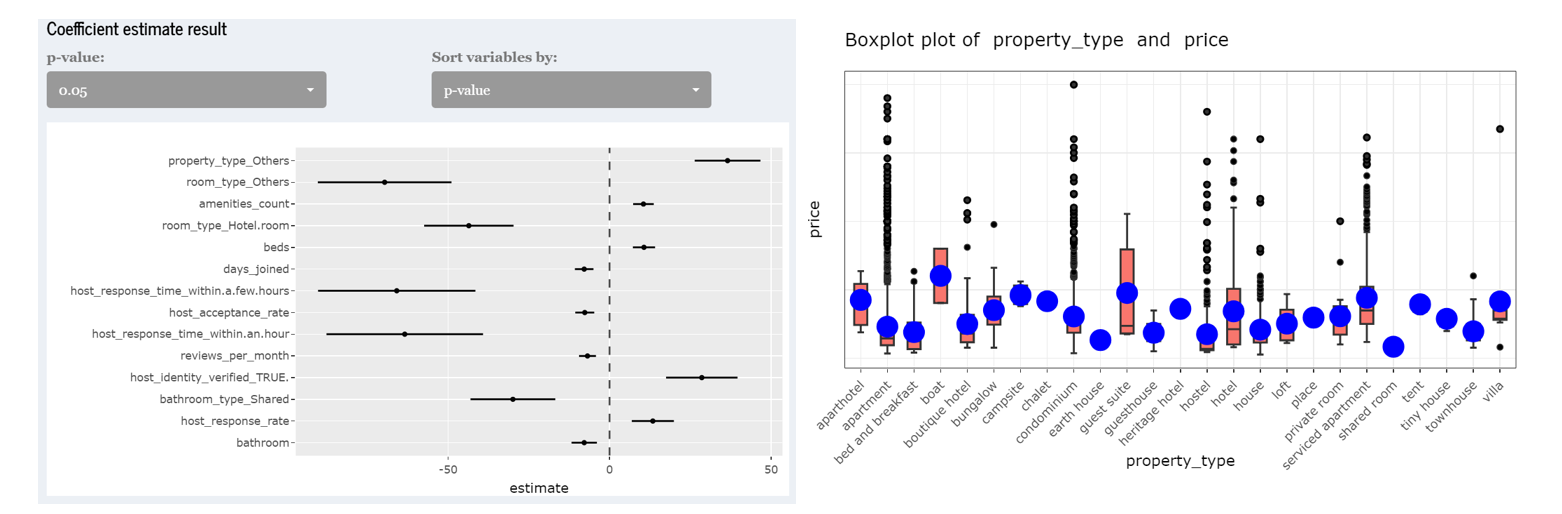
\includegraphics[width=1\linewidth]{images/LMcoeff} 

}

\caption{Coefficient estimate and boxplot from exploratory module}\label{fig:unnamed-chunk-21}
\end{figure}

\hypertarget{discussion}{%
\section{Discussion}\label{discussion}}

In this project, we have developed ShinyPET, an interactive web-based
application to promote data exploratory, text analytics and predictive
analytics on Airbnb data set. The interactivity and functionality of our
application provides evidence on the robustness of R shiny as a
framework to develop web application, along with the variety of
available R packages that serve as building blocks for each module in
our application. On top of the functionality, user interface is also
carefully designed with the arrangement of submodules for each analytics
task, to ease the usage for non-technical user. With the integration of
main analytics task (exploratory, textual, and predictive), our
application enables user to assess and make use of a dataset from
different perspective in a single platform. The modularisation of
analytics task allows user to quickly navigate between modules when
necessary. Example of benefit from such case has been discussed
previously where exploratory module can aid in the understanding of
predictive model.

\hypertarget{future-work}{%
\section{Future Work}\label{future-work}}

Shiny PET was built in relation to Singapore's Airbnb dataset as a
usecase. The Shiny PET enable users to perform exploratory and
confirmatory analysis, text mining, and predictive modelling without
users needing extensive programming or statistical knowledge. The
application could be further enhance by including a data load and
wrangling function to accommodate different datasets.

The current types of chart and statistical test are limited to only 4
types of charts and parametric statistical test for each chart type
respectively. Other charts, such as violin and bar charts, can be
incorporated further. Additional hypothesis testing methods such as
non-parametric test for median, statistical test by pairs etc. can be
incorporated. The current application supports two types of map,
providing room for additions in terms of kernel density map and
navigation map.

Additionally, token frequencies and sentiment analysis allow selection
of n-grams and lexicons respectively. Further interactivity such as
choices of neighbourhood, rating scores can be added. Moreover, the
explore and text sub modules can be connected with views coordinated and
linked in order to provide multiple dimensional exploration.

The current predictive module is limited to 5 types of predictive model.
More predictive models e.g.~neural network can be to provide users with
wider model selection. In hyper-parameter tuning, parameters can be made
available for user input to provide more flexibility in developing
predictive model. In-depth statistical analysis in model training such
as residual analysis are currently not available and this would be a
good additional tool to improve our application.

\hypertarget{acknowledgement}{%
\section{Acknowledgement}\label{acknowledgement}}

The authors wish to thank Professor Kam Tin Seong of Singapore
Management University for his extensive guidance and support during this
project.

\hypertarget{references}{%
\section*{References}\label{references}}
\addcontentsline{toc}{section}{References}

\hypertarget{refs}{}
\begin{CSLReferences}{0}{0}
\leavevmode\vadjust pre{\hypertarget{ref-airbnb2021}{}}%
\CSLLeftMargin{{[}1{]} }
\CSLRightInline{Curry, D. 2021. \emph{Airbnb revenue and usage
statistics}.}

\leavevmode\vadjust pre{\hypertarget{ref-harris_2014}{}}%
\CSLLeftMargin{{[}2{]} }
\CSLRightInline{Harris, J. 2014. Data is useless without the skills to
analyze it. \emph{Harvard Business Review}.}

\leavevmode\vadjust pre{\hypertarget{ref-tidymodels2020}{}}%
\CSLLeftMargin{{[}3{]} }
\CSLRightInline{Kuhn, M. and Wickham, H. 2020. \emph{Tidymodels: A
collection of packages for modeling and machine learning using tidyverse
principles.}}

\leavevmode\vadjust pre{\hypertarget{ref-https:ux2fux2fdoi.orgux2f10.1111ux2fcgf.13210}{}}%
\CSLLeftMargin{{[}4{]} }
\CSLRightInline{Lu, Y. et al. 2017. The state-of-the-art in predictive
visual analytics. \emph{Computer Graphics Forum}. 36, 3 (2017),
539--562.}

\leavevmode\vadjust pre{\hypertarget{ref-doi:10.1080ux2f00461520.2012.667064}{}}%
\CSLLeftMargin{{[}5{]} }
\CSLRightInline{Mandinach, E.B. 2012. A perfect time for data use: Using
data-driven decision making to inform practice. \emph{Educational
Psychologist}. 47, 2 (2012), 71--85.}

\leavevmode\vadjust pre{\hypertarget{ref-radiant2019}{}}%
\CSLLeftMargin{{[}6{]} }
\CSLRightInline{Nijs, V. 2019. \emph{Radiant -- business analytics using
r and shiny}.}

\leavevmode\vadjust pre{\hypertarget{ref-robinson}{}}%
\CSLLeftMargin{{[}7{]} }
\CSLRightInline{Robinson, J.S. and David Text mining with r: A tidy
approach. \emph{Welcome to Text Mining with R \textbar{} Text Mining
with R}.}

\leavevmode\vadjust pre{\hypertarget{ref-https:ux2fux2fdoi.orgux2f10.1016ux2fj.jbusres.2020.03.028}{}}%
\CSLLeftMargin{{[}8{]} }
\CSLRightInline{Yasmin, M. et al. 2020. Big data analytics capabilities
and firm performance: An integrated MCDM approach. \emph{Business
Research}. 114, (2020), 1--15.}

\end{CSLReferences}
\setlength{\parindent}{0in}

\end{document}
